

% \documentclass{beamer}
% \usepackage[utf8]{inputenc}
% \mode<presentation> {

% The Beamer class comes with a number of default slide themes
% which change the colors and layouts of slides. Below this is a list
% of all the themes, uncomment each in turn to see what they look like.

%\usetheme{default}
%\usetheme{AnnArbor}
%\usetheme{Antibes}
%\usetheme{Bergen}
%\usetheme{Berkeley}
%\usetheme{Berlin}
%\usetheme{Boadilla}
%\usetheme{CambridgeUS}
%\usetheme{Copenhagen}
%\usetheme{Darmstadt}
%\usetheme{Dresden}
%\usetheme{Frankfurt}
%\usetheme{Goettingen}
%\usetheme{Hannover}
%\usetheme{Ilmenau}
%\usetheme{JuanLesPins}
%\usetheme{Luebeck}
% \usetheme{Madrid}
%\usetheme{Malmoe}
%\usetheme{Marburg}
%\usetheme{Montpellier}
%\usetheme{PaloAlto}
%\usetheme{Pittsburgh}
%\usetheme{Rochester}
%\usetheme{Singapore}
%\usetheme{Szeged}
%\usetheme{Warsaw}

% As well as themes, the Beamer class has a number of color themes
% for any slide theme. Uncomment each of these in turn to see how it
% changes the colors of your current slide theme.

%\usecolortheme{albatross}
%\usecolortheme{beaver}
%\usecolortheme{beetle}
%\usecolortheme{crane}
%\usecolortheme{dolphin}
%\usecolortheme{dove}
%\usecolortheme{fly}
%\usecolortheme{lily}
%\usecolortheme{orchid}
%\usecolortheme{rose}
%\usecolortheme{seagull}
%\usecolortheme{seahorse}
%\usecolortheme{whale}
%\usecolortheme{wolverine}

%\setbeamertemplate{footline} % To remove the footer line in all slides uncomment this line
%\setbeamertemplate{footline}[page number] % To replace the footer line in all slides with a simple slide count uncomment this line

%\setbeamertemplate{navigation symbols}{} % To remove the navigation symbols from the bottom of all slides uncomment this line
% }

% \usepackage{graphicx} % Allows including images
% \usepackage{booktabs} % Allows the use of \toprule, \midrule and \bottomrule in tables

% %----------------------------------------------------------------------------------------
% %	TITLE PAGE
% %----------------------------------------------------------------------------------------

% \title[Short title]{Main Topic } % The short title appears at the bottom of every slide, the full title is only on the title page

% \author{John Smith} % Your name
% \institute[UCLA] % Your institution as it will appear on the bottom of every slide, may be shorthand to save space
% {
% University of California \\ % Your institution for the title page
% \medskip
% \textit{john@smith.com} % Your email address
% }
% \date{\today} % Date, can be changed to a custom date

% \begin{document}

% \begin{frame}
% \titlepage % Print the title page as the first slide
% \end{frame}

% \begin{frame}
% \frametitle{Overview} % Table of contents slide, comment this block out to remove it
% \tableofcontents % Throughout your presentation, if you choose to use \section{} and \subsection{} commands, these will automatically be printed on this slide as an overview of your presentation
% \end{frame}

\section{Problématique et modèle} 
\subsection{Problème}

\begin{frame}{Problème}
Réduire les dépenses du terminal sud :
\begin{center}
    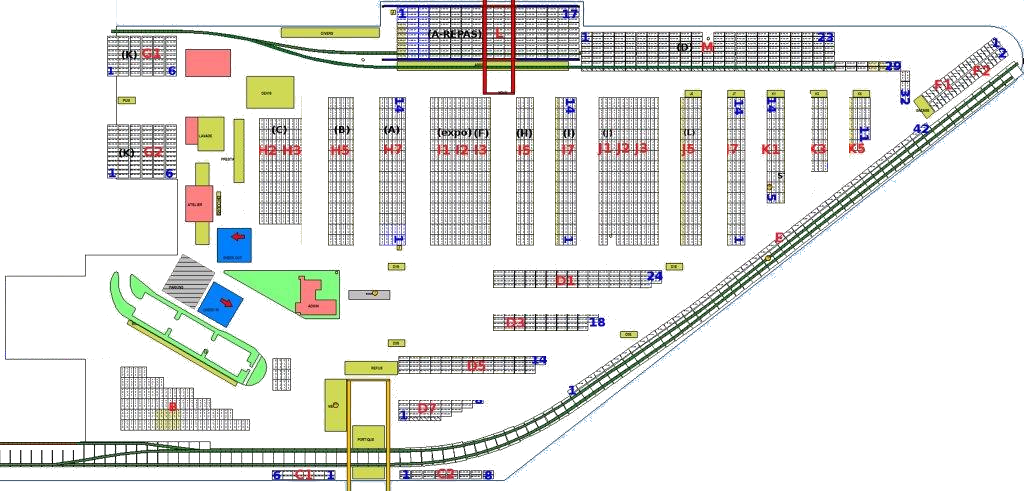
\includegraphics[scale=0.5]{../images/Plan_Terminal.png}
\end{center}

\end{frame}
 

\subsection{Hypothèses}

\subsection{Quelques termes techniques}
\begin{frame}{Quelques termes techniques}
  \vfill
       \begin{itemize}
       \item Travée, pile, bloc, allée, zone de chargement.
        \vfill
       
   \item Géométrie : répartition des emplacements sur le terminal.
   \vfill
   \item Client.
        
      
    \vfill
    \item Configuration : une répartition des conteneurs pour une géométrie fixée.
      
 
\end{itemize}
\vfill
\end{frame}

\begin{frame}{Hypothèses}

\begin{itemize}
\vfill
    \item se restreindre aux conteneurs 20 pieds,
    \vfill
    \item effectuer une étude 2D,
    \vfill
     \item utiliser une seule zone de chargement.
    \vfill
\end{itemize}
 \vfill
\end{frame}

\subsection{modèle}

\begin{frame}{Idée}
\begin{center}
    Minimiser la distance parcourue par un conteneur en fonction de la géométrie et de la configuration.
\end{center}

    
\end{frame}

\begin{frame}{Données statistiques}
Extraits à partir de données statistiques : 
\begin{itemize}
 \vfill
    \item $\mu_c$ : poids du client $c$,
 \vfill
    \item $V_{tot}$ : nombre total de conteneurs (4500 EVP),
     \vfill
       \item  $V_c$ : nombre "moyen" de conteneurs stoqués sur le port par le client $c$.
\end{itemize}
 \vfill


\end{frame}



\begin{frame}{Contraintes sur la géométrie}
\vfill 
\begin{itemize}
    \item $N_t$ : largeur de la travée $t$.
\end{itemize} 
\vfill
Contraintes : 
  \vfill
\begin{itemize}
 \item $1 \leq N_t \leq 15$,
    \vfill
    \item $\mathrm{Card}(N_t\vert N_t \geq  6) \leq  30$,
    \vfill
     \item la largeur d'une allée est supérieure à $15m$.
     \vfill
   
\end{itemize}   
  \vfill

    
\end{frame}




\begin{frame}{Géométrie et distances}
\vfill
\begin{itemize}
    \item $d_t$ : distance associée à une travée $t$ pour une géométrie fixée.
    \vfill
    \item $d_{t,E1}$ : distance entre la travée $t$ et l'entrée $1$.
    \vfill
    \item $d_{t,E2}$ :  distance entre la travée $t$ et l'entrée $2$.
    \vfill
    \item $d_{t,z}$ :  distance entre la travée $t$ et la zone de chargement.
    
\end{itemize}
\vfill
     $$d_t=\frac{2}{3}d_{t,E1}+\frac{1}{3}d_{t,E2}+d_{t,z}.$$


    \vfill
\end{frame}

\begin{frame}{Configuration}

   \begin{itemize}
       \item  $x_{t,c}$ : nombre d'emplacements utilisés par le client dans la travée $t$.
   \end{itemize} 
   
   \vfill Contrainte : 
   
   \vfill
   \begin{itemize}
   
       \item $x_{t,c}x_{t,c'}=0,\quad \forall t \quad \forall c\neq c'$ : un travée est utilisée par un seul client.
       \end{itemize}
   \vfill
  
\end{frame}




\begin{frame}{La fonction coût}
\vfill
\begin{itemize}
    \item  La fonction coût  : 
    \vfill
    $$ \sum_t \sum_c d_t* \mu_c* x_{t,c}.  $$
      \vfill
     \item La fonction coût correspond à la distance moyenne parcourue par un conteneur.
\end{itemize}
     \vfill
\end{frame}

\begin{frame}{Optimisation}

\vfill
\begin{itemize}
    \item L'objectif est de minimiser la fonction coût en fonction de la géométrie et de la configuration.
     \vfill
     \item  L'idéal serait de pouvoir générer des géométries et des configurations, puis de comparer les différentes valeurs des fonctions coût. 
     
\end{itemize}
     \vfill
    
\end{frame}

% \end{document}